\section{Methods -- Experiment One: Choosing among Independent Options}~\label{method_exp1}

We designed a between-subjects randomized controlled experiment to answer our first research question: \begin{quote} RQ1: How do QV responses align with people's true preferences compared to Likert scale responses in a survey where survey respondents choose among $K$ independent options of one topic? How do variations in the number of voice credits given to QV survey respondents impact this outcome? \end{quote} The study was in the context of a public opinion polling to understand participants' preferences towards various societal causes, such as the environment, education, veteran. We focused on the topic of societal causes because public goods and resource allocation across causes is a problem relevant to every citizen. Since resources are limited in public sectors, this problem is a typical example of choosing among $K$ independent options. Each participant completed one of the two kinds of surveys on the importance of the nine societal causes and a donation task. We detail the flow of our experiment in this section.

\subsection{Participants Recruitment}
We recruited participants located in the US from Amazon Mechanical Turk (MTurk) through the CloudResearch platform \cite{litman2017turkprime}. We made our best efforts to align the participants' age and education level distribution to the 2018 United States census estimates \cite{census2018}. We randomly assigned them into two groups: the Likert group and the QV group. Participants in the Likert group had a median completion time of 11.5 minutes and received \$0.75, and those in the QV group received \$2.5 due to a longer study length, with a median completion time of 20 minutes 56 seconds.

\subsection{Experimental Flow}
\begin{figure}[htpb]
    \centering
    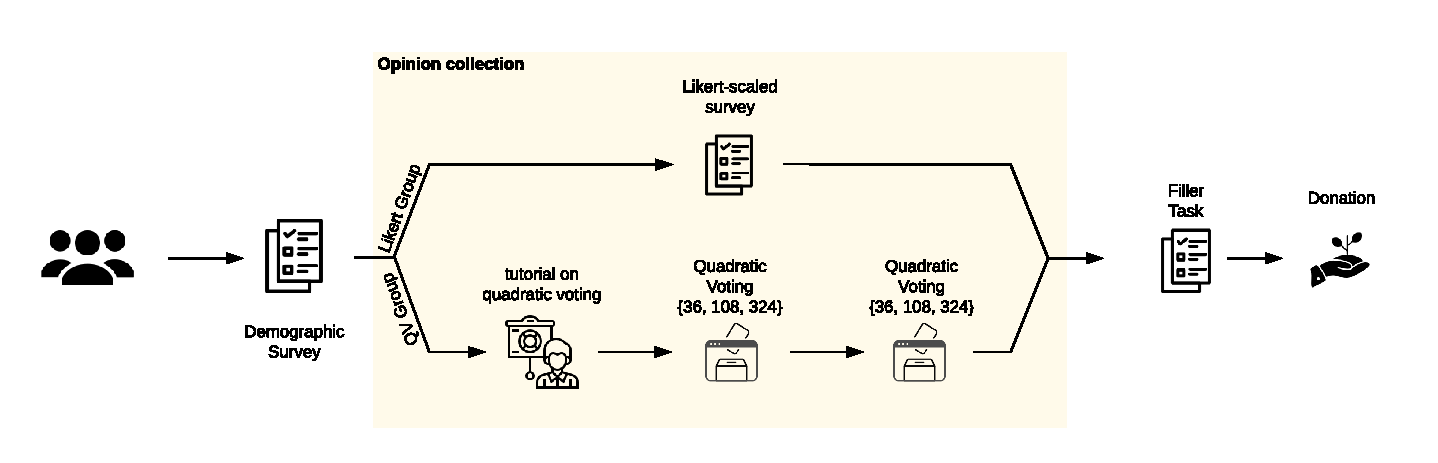
\includegraphics[width=\textwidth, keepaspectratio=true]{content/image/exp1_flow.pdf}
    \caption{
        Experiment one was a between-subjects experiment. We randomly assigned participants into two groups. Participants that took the upper path were in the Likert Group, and they expressed their attitudes toward various social causes through a five-point Likert scale. QV group participants reported their attitudes through two of the three variations of QV survey, with $36$, $108$, and $324$ voice credits respectively.
    }
    \label{fig:exp1_image_flow}
\end{figure}

\Cref{fig:exp1_image_flow} summarizes the experimental procedure. The experiment consisted of four steps: 1) demographic survey, 2) Likert or QV survey, 3) distraction survey, and 4) donation task. We provide the complete experimental protocol in the supplementary materials.

% Participants filled out the demographic survey as the first step. Based on the demographics, participants completed one or more surveys, as highlighted in the figure. Participants in the Likert group filled out one Likert survey, while participants in the QV group completed two QV surveys. After that, participants filled out another survey, the distraction survey, to divert their attention before completing the final task. We ask participants to donate to a list of charities. We explain each of these steps in detail.

% \begin{enumerate}[label=\textbf{Step }\arabic{*}\textbf{:}, leftmargin=0.45in]

\textbf{Step 1: Demographic Survey.} Participants joined the study under the impression that the goal of the study was to understand their opinions towards \textit{the importance of various societal causes}. After signing the consent form, participants completed a demographic survey that asked for their gender, ethnicity, age, household income level, education level, and current occupation.

\textbf{Step 2.1: Group 1 -- Likert Scale Survey.} The experiment randomly assigned some of the participants to the Likert group, shown in the upper path of \Cref{fig:exp1_image_flow}. In the prompt, we explicitly told the participants that there are limited resources in the society, and people have different preferences at allocating resources to various societal causes. The survey focused on nine societal issues, including 1) pets and animals, 2) arts, culture and humanities, 3) education, 4) environment, 5) health, 6) human services, 7) international causes, 8) faith and spiritual causes, and 9) veteran\footnote{For detailed definitions of each cause, please refer to~\Cref{cause_def}}. We derived the nine societal causes from the categorization of charity groups on Amazon Smile \footnote{https://smile.amazon.com/}, a popular donation website that has accumulated over 100 million dollars of donations.

We asked the participants to rate each of the nine societal issues on a 5-point Likert scale: ``For each of the issues listed below, how important do you think the issue is to you and that more effort and resources should be contributed towards the issue?''. The 5-point Likert options ranged from ``Very important'' to ``Very Unimportant.'' While there are a variety of Likert scales (3-point, 5-point, 7-point, and even 11-point), we used a 5-point Likert scale since it is one of the most commonly used scale \cite{dawes2008data}.

\textbf{Step 2.2: Group 2 -- QV Survey} The QV group took the lower path in \Cref{fig:exp1_image_flow}. We first asked participants to watch a pre-recorded tutorial video that introduced how QV works and how to use our QV interface since we did not expect participants to know about QV before taking part in the study, as opposed to Likert scale. Participants had unlimited time to interact with a demo QV interface to familiarize themselves with QV. To ensure that the participants paid attention and understood QV, they needed to correctly answer at least three of the five multiple-choice quiz questions related to QV to continue with the study.

Once they passed the quiz, participants encountered two of the three versions of the QV surveys at random. The three versions of QV had 36, 108, and 324 voice credits, respectively. We showed them the same prompt as in the Likert group and instructed them to answer the same question for the nine identical causes, but with QV instead. Participants cast positive votes for causes they considered important and vice versa.
% They vote in QV using these voice credits on the nine identical options presented to the Likert Group. Participants would repeat this action using a different voice credit. We show these two QV surveys as two QV icons in \Cref{fig:exp1_image_flow}.

To our knowledge, no prior work discussed about how to decide on the voice credit budget in QV empirically. Therefore, we designed three versions of the QV survey to answer the second question in RQ1: how does the amount of voice credits in QV impact QV's ability to elicit true preferences? To examine how larger voice credit budgets impact people's choices, we set an exponential increase based on the number of options ($K$) on the survey ($O(K)$, $O(K^{1.5})$ to $O(K^2)$). We investigated three levels of voice credits: $K \times O$, $K^{1.5} \times O$, and $K^2 \times O$, where $K$ is the number of options in the survey and $O$ is the number of credits required to express an attitude in QV that is equivalent to the strongest attitude in a 5-point Likert scale survey, where ``Neutral" in Likert = 0 vote in QV and one level in Likert = one vote in QV. In this experiment, $K=9$ corresponded to the $9$ societal causes. We used a 5-point Likert scale survey with extreme levels at $+/-2$; hence the participant need four voice credits ($2^2=4$) to express the extreme Likert levels in QV, which translated to $O=4$. Thus, the three levels of voice credits in the experiment were $36$ (QV36), $108$ (QV108), and $324$ (QV324). In all three cases, participants could afford to express any results from Likert in the form of QV. 


\textbf{Step 3: Distraction Survey} After both groups of participants completed their surveys on the nine societal causes, they answered a free-form text question about their thoughts on another set of societal issues unrelated to those presented in the previous stage, such as increasing funding for Medicaid, strengthening gun control, and tighten social media regulation. For a complete list of causes, please refer to the supplementary material. We intentionally designed this survey to prevent participants from directly connecting their survey responses with the upcoming donation tasks. 

\textbf{Step 4: Donation Task} In the last step of the experiment, we need to design an incentive-compatible mechanism to elicit participants' true preferences towards the societal causes in the QV and Likert scale surveys. We designed a voluntary donation task with lottery-incentives, where their donation amount should reflect how much they truly care about the causes. In this task, to the best of their interest, they should donate more to organization A than organization B only if they care more about the cause of organization A. 

We believe voluntary donation was a suitable task to collect the participants' truthful preferences for three reasons. First, many prior work \cite{Xiao2019, benz2008people, gendall2010effect, hsieh2010pay, hsieh2016you} used donation as an indicator of participants' preferences. Second, voluntary donation is ecologically valid, a task that occurs in real-life settings. Lastly, donation does not require specialized knowledge and is simple to conduct online and at scale. We now describe how our donation mechanism worked.

We showed participants a list of nine charities in a randomized order with an introduction and an official website. We selected one charity for each of the nine societal causes in the QV and Likert scale surveys via Amazon Smile. But we chose not to show their mapping to the causes explicitly to the participants to maintain as much independence between the survey responses and the donation decisions as possible. 

Participants had the chance to win \$35 as a bonus through a lottery with an odds of 1 in 70. We asked them whether they would like to donate part of this bonus to any of the nine charity groups if they were the winner. They would keep the remaining amount after the donation to themselves. While participants could donate any amount to any organization as long as the total donation value did not exceed \$35, they would want to maximize their bonus, which encouraged them to be truthful about the amount to donate. To increase participants' chance of donating a non-zero total amount, the research team promised to match \$1 to each dollar they donated to an organization and execute the donation on their behalf if they won the lottery. 
% This setup meant that the donation behavior carried an underlying cost.

% Fourth, donating is a behavior that contains complimentary and homogenous choices, and each of the options is independent. The donation task is a clear example of choosing one out of $K$ in a real-life setting.
% Adult individuals regularly exercise monetary behaviors and make financial decisions daily. These characteristics of the donation task mean that participants should not have challenges completing this task. 

% To minimize the difference across groups in the study, we used the same prompt across the Likert survey, QV, and the donation task. We explicitly told the participants that there are limited resources in society, and people have different preferences at allocating resources. We asked the participants, 
% ``What societal issues need more support?'' across all our surveys.

% \end{enumerate}

\subsection{System Design}

\begin{figure}[htpb]
    \centering
    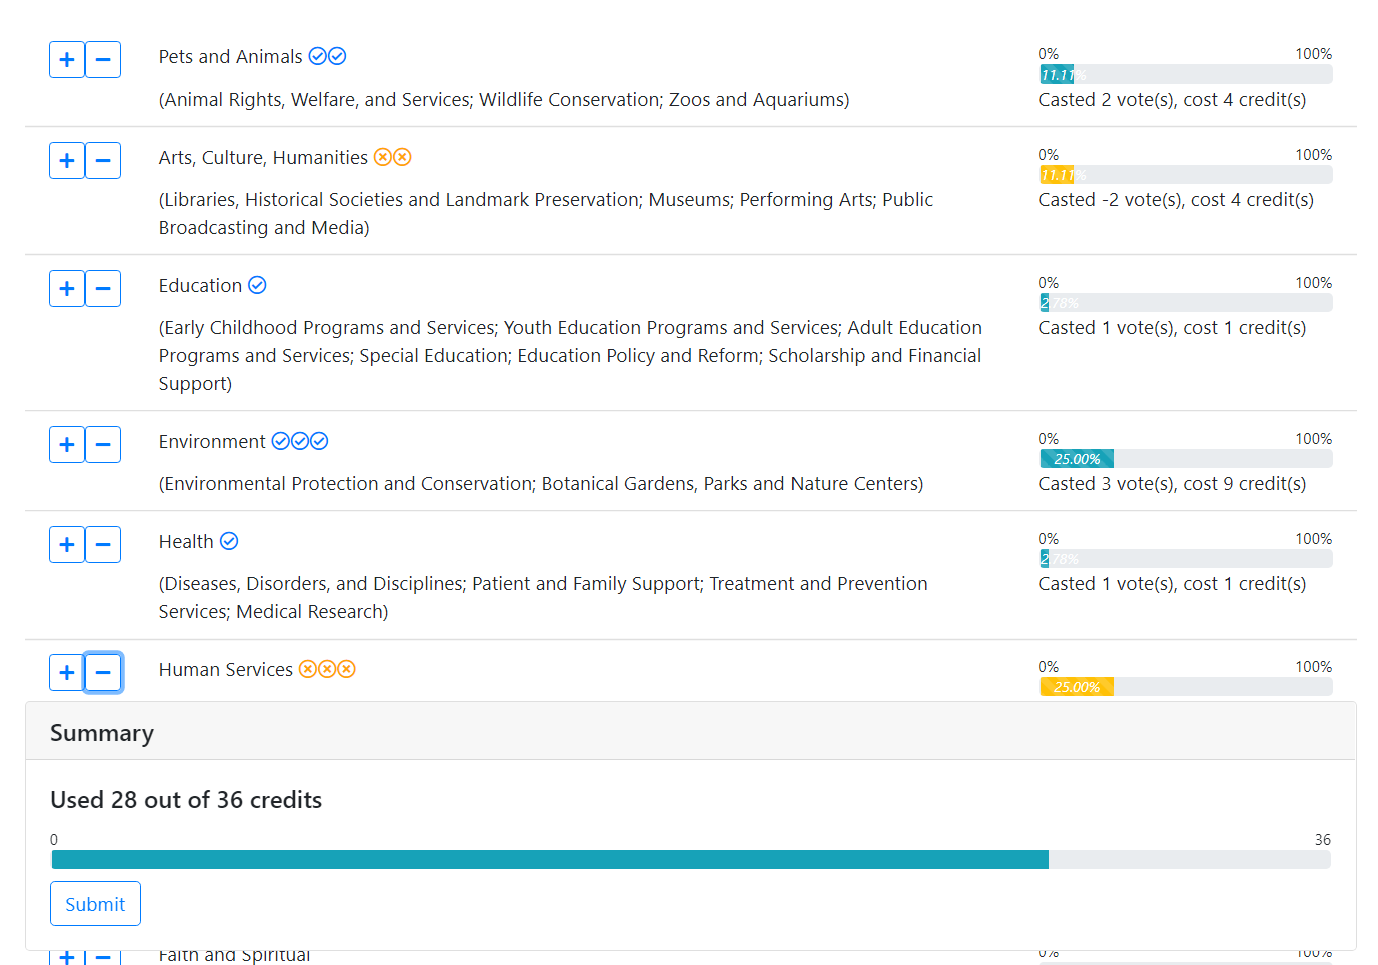
\includegraphics[width=0.7\textwidth, keepaspectratio=true]{content/image/qv-donation.png}
    \caption{
        Our QV interface design in the experiments. 
        We omitted the prompt in this figure.
        After multiple design iterations, 
        the final interface allows participants to vote, with real-time feedback of how the credits are allocated. 
        The progress bar design was inspired by the knapsack voting interface by \cite{goel2015knapsack}.
    }
    \label{fig:qv_donation}
\end{figure}

We designed the QV interface through iterative-design (process detailed in \Cref{appx_qv_interface}) with the goal to reduce participants' cognitive load with visual information \cite{oviatt2006human}. \Cref{fig:qv_donation} shows the body section of the voting panel that contained a list of options to vote on. To the left of each option, participants voted using the plus and minus buttons. Buttons for an item were automatically disabled if the number of voice credits remaining did not permit an additional vote for that item. The number of blue check or yellow cross icons next to the item represented the number of ``for'' and ``against'' votes. We provided participants a bar with percentages to the right of each option, which showed the proportion of voice credits used for that option.  In the summary panel, a progress bar showed the number of voice credits the participants have and have not used out of the total budget. We floated the summary panel at the bottom of the page at anytime to ensure visibility.

For our experimental system, we used Angular.js for the front-end, Python Flask for the back-end implementation, and MongoDB Atlas for the database. The experimental system source code is publicly available \footnote{https://github.com/dummy\_url}, and so is the code for the standalone QV interface \footnote{https://github.com/dummy\_url}. 
% The QV interface repository is a stand-alone repository written in Angular and Flask.



% -- data transformation to alignment measurement
%     describe the calculation of cosine similarity angle theta
%     mention our test of checking if other factors impact total donation amount -> absolute vs. normalized donation amount
%     show histogram and other descriptive statistics of the angle data
\subsection{Analysis Method -- Opinions Alignment Metric}~\label{alignment_metric}

We break our research question on ``alignments'' into two parts. First, we ask how similar these individual survey responses are to a participant's incentive-compatible behavior. Then we ask, how does QV and Likert compare overall in terms of the degree of alignment? To answer the first question, we need a metric for alignment.

We first clarify the definition of "alignment" in our analysis. A perfect alignment between a survey response and the same participant's donation choices requires an individual to express their preferences in survey with the same relative strength as their donation amount. More formally, it is defined as the following:

\begin{quote}
    A set of survey response $\vec{v} = (v_1, v_2, \dots, v_n) \in \mathbb{R}^n$, and a set of donation amount $\vec{d} = (d_1, d_2, \dots, d_n)\in \mathbb{R}_{+}^n$, where $n$ is the number of topics or options involved in the decision, are perfectly aligned if there exists a positive constant $k>0$ that satisfies $k\vec{v} = \vec{d}$.
\end{quote}

Notice now we represent the a participant's response in Likert scale survey, QV, and donation each with a vector of the same length. In addition, we focus the definition of alignment on the \textit{relative} strength across opinions for two reasons. First, the results from our four types of surveys (Likert, QV36, QV108, QV324) and the donation task were not on the same scale. For example, the maximum possible number of votes on a topic in QV36 was 6, while the maximum donation amount on a topic was \$35. A relative scale maps each response onto the same space. The other reason is when any two participants donated different absolute amounts, possibly due to other factors such as income level or level of education, we want to capture how they \textit{distributed} their total donation amounts. In other words, participants might donate with the \textit{same} set of preferences across topics, but with \textit{different} levels of total amount they were willing to donate. Hence, we decided to care only about the relative strength in opinions across topics.

Next, we need a metric that measures the degree of alignment. This metric needs to be monotonic with respect to the amount of discrepancy between two preference vectors in terms of the relative strength across preferences. In addition, this metric needs to be easily interpretable. Therefore, we decided to make use of the cosine similarity metric as our alignment metric and represent the difference between the survey results and the donation amount with an angle $\theta$. It is formally defined as the following:

\begin{quote}
    The cosine similarity angle $\theta$ between a set of survey response $\vec{v} = (v_1, v_2,\dots, v_n) \in \mathbb{R}^n$, and a set of donation amount $\vec{d} = (d_1, d_2,\dots, d_n) \in \mathbb{R}_{+}^n$, where $n$ is the number of topics or options involved in the decision, is calculated via $\theta = \arccos \left ( {\frac{\langle \vec{v},  \vec{d} \rangle}{\|\vec{v}\| \|\vec{d}\|}} \right )$, $\theta \in (0, \pi)$.
\end{quote}

Cosine similarity is a commonly used similarity metric 
that measures the cosine of the angle between two non-zero vectors \cite{singhal2001modern}. Instead of reporting a value between $0$ and $2 \pi$ radians, we report the angle in degrees, allowing for a more intuitive interpretation.
%The definition of the angle of Cosine similarity fits our need perfectly. 
It is monotonic with respect to the relative orientations of the two vectors, i.e., the relative strength in opinions, and does not take into account the magnitude of the vectors, i.e., absolute vote or donation amount. Two sets of perfectly align opinions will yield a cosine similarity angle of zero, while two sets of completely opposite opinions will result in an angle of 180 degree.

% Intuitively,
% to compute the Cosine similarity angle 
% for each participant in each group,
% we first translate each response,
% urvey results from Likert, QV36, QV108, QV324, and 
% their corresponding truthful preferences 
% reflected in the donation task,
% into a vector. %mentioned above can repeat if necessary
For the Likert group, we map the ordinal responses into a vector where the result for each topic ranges from $-2$ to $2$. For each of the three QV conditions, the vector contains the number of votes of the topics as is. Then, for each individual, we computed the cosine similarity angle between the Likert or QV vector and the absolute donation amount of the same individual. 

Once we gathered these data, we moved on to the next step where we uncovered how the cosine similarity angles compared across the Likert group and the three QV variances (QV36, QV108 and QV324). We set up a Bayesian Model with these four sets of cosine similarity angle for each condition, as described in the next subsection.

\subsection{Analysis Method -- A Bayesian Approach}
\label{exp1:The Bayesian Model}


% In many survey analysis experiments, researchers relied heavily on the null hypothesis statistical tests (NHST) to determine whether a phenomenon is statistically significant or not, to support their hypothesis. This method leads to controversies in the field for a very long time. One major challenge of NHST came from its goal: rejecting the null hypothesis. Instead of answering the alternative directly, this made NHST easy to overstate the evidence against the null hypothesis \cite{david2000NHST}. In addition, some researchers \cite{kruschke2010bayesian} argued that it is easy to `p-hack' an experiment by replicating an experiment repetitively and only reporting the ones with significant results. There were heated debates upon confidence intervals, alpha values, the sample size decision, and many others when discussing related issues of NHST.

We used Bayesian analysis to compare if the distribution of cosine similarity angle in the QV group significantly differs from that in the Likert group. The core concept of Bayesian analysis is updating and reallocating the belief as one gathered more information with the use of Bayes rules. Kay et al. \cite{kay2016researcher} introduced the following benefits of using this analysis method in the HCI community. First, Bayesian shifts the conversation from ``did it work" to ``how strong is the effect." While null hypothesis statistical tests (NHST) produces a single p-value and one effect size value, a Bayesian model can provide the distribution of the effect size, making additional information available for a clear inference. Second, a Bayesian model is valid at every value of the sample size while NHST that assumes normality requires at least a sample size of 30. Lastly, a Bayesian model does not require the assumptions of normality and homogeneity of variance since the researcher can foreground all the aspects of the model. 


Now, we discuss our Bayesian formulation. There is one outcome variable: $\theta_{i \mid j}$, the cosine similarity angle between a survey response vector and a donation amount vector of each participant $i$  under each of the four experimental conditions $j$: Likert, and three QV conditions (with 36, 108 and 324 credits). In summary, we aim to fit a distribution for the mean (i.e. the expected) angle between responses from each survey method and the donation amount. Then we compare how different the four distributions are. 

In a Bayesian formulation, we need to define a likelihood function to model the cosine similarity under each condition. In general, this is a parametric formulation, and consistent with~\textcite{McElreath2015}. The likelihood function represents the modeler's view of the data, and not a claim about the world. The likelihood function is often parametric and we treat each model parameter as a random variable, drawn from a distribution (its prior). Typically, these priors are ``weakly informative''---conservative priors which allow for all possible values of the parameter but chosen in a manner that promotes fast convergence.


We use a Student-t distribution to characterize the mean (i.e. the expected) angle in all four survey conditions (Likert and the three QV conditions). A Student-t, unlike a Normal distribution, is heavy-tailed, in the sense that the Student-t distribution doesn't fall off as quickly as does a Normal distribution and will thus be able to better account for outliers in the data. The Student-t distribution has three parameters: the degrees of freedom ($\nu$), the experimental condition dependent mean ($\mu_j$) and scale ($\sigma_j$).  These parameters are random variables and we need to define their priors. Since our goal is to model the \textit{average} angle, the fact that the Student-t is unbounded while the angle $\theta \in [0, \pi]$ is bounded is unimportant.

\begin{align}
  \theta_{i \mid j} \sim & \mathrm{Student-t}(\nu, \mu_j, \sigma_j),   & \text{likelihood function to model donation} \label{eq:bayesian formulation} \\
  \nu \sim & 1 + exp(\lambda), & \text{degrees of freedom} \\
  \mu_j \sim & N(M_0, \sigma_0), & \text{modal angle in condition } j \\
  \sigma_j \sim & \Gamma(\alpha, \beta), & \text{scale parameter for condition } j
\end{align}
 
\Cref{eq:bayesian formulation} describes that the response $\theta_{i \mid j}$ of each group $j$ is modeled as a $\mathrm{Student-t}$ distribution with mode $\mu_j$,  scale $\sigma_j$ and with $\nu$ degrees of freedom. Next, we explain the model parameters.


\begin{description}
    \item[Degrees of Freedom:] We draw the degrees of freedom $\nu$ from a shifted exponential distribution, to ensure $\nu \geq 1$; $\nu=\infty$, corresponds to a Normal distribution assumption.
    \item[Modal contribution $\mu_j$ in each condition $j$:] The mode $\mu_j$ corresponding to each group is drawn from a Normally distributed random variables with constant mean $M_0$ and variance $\sigma_0$. 
    \item[Scale $\sigma_j$ of each condition $j$:]  The scale $\sigma_j$ of the likelihood function is drawn from a Gamma distribution $\Gamma(\alpha, \beta)$, with mode $\alpha$ and scale $\beta$; this prior on $\sigma_j$ ensures that $\sigma_j > 0$. 
    \item[Constants:] The constants $M_0, \sigma_0, \alpha, \beta$ are set so that the priors are generous but weakly informative so that despite exploring all possible values, we ensure rapid MCMC convergence.
\end{description}

We performed the Bayesian analysis using PyMC3 \cite{salvatier2016probabilistic}, 
a popular Bayesian inference framework. We used one of the common computational techniques for Bayesian inference, Markov Chain Monte Carlo (MCMC), a stochastic sampling technique. It samples the posterior distribution $P(\theta | D)$, the distribution functions of the parameters in the likelihood function given the data observations $D$. 
% We used the No-U Turn Sampler (NUTS) specifically 
% in our analysis. 


%% Old draft text
% % Experiment overview
% We designed the first experiment as a between within-subject study
% consisting of Likert survey, QV, and a donation task,
% to answer research questions one and three. 
% Participants were recruited from Amazon Mechanical Turk (MTurk).
% The Likert Group received \$0.75 
% while the QV and Likert Group received \$1.75 
% when participants completed the study.
% In this section, 
% we detailed our experiment design.

% The goal of a between within-subject study is to
% understand how within-subject does a survey tool
% aligns with one's true preference.
% To compare QV and Likert, 
% these results, 
% the difference between the survey tool and one's preference, 
% were then compared across groups of participants.

% %The donation task. Why?
% In order to figure out 
% how QV and Likert surveys 
% represent an individual's true preferences,
% we ask participants to complete a survey
% and donate to a charity.
% Our goal is to see 
% whether a participant's donation behavior is similar to 
% the attitudes they stated in the survey.
% There are multiple reasons
% why we designed a donation task.
% First, donation tasks are easily relatable
% given that they occur in real life and
% and monetary behaviors are direct and imaginable.
% Second, donations are simple to conduct,
% even on a large scale.
% Third, donation tasks appeared in many experiments 
% \cite{Xiao2019, benz2008people, gendall2010effect} 
% as an effective indicator of participants' behavior.
% Fourth, donating is a behavior containing
% complimentary and homogenous choices and
% where each of the options is independent.
% It is a clear example of choosing one out of $K$ in real life.

% \begin{figure}[htpb]
%     \centering
%     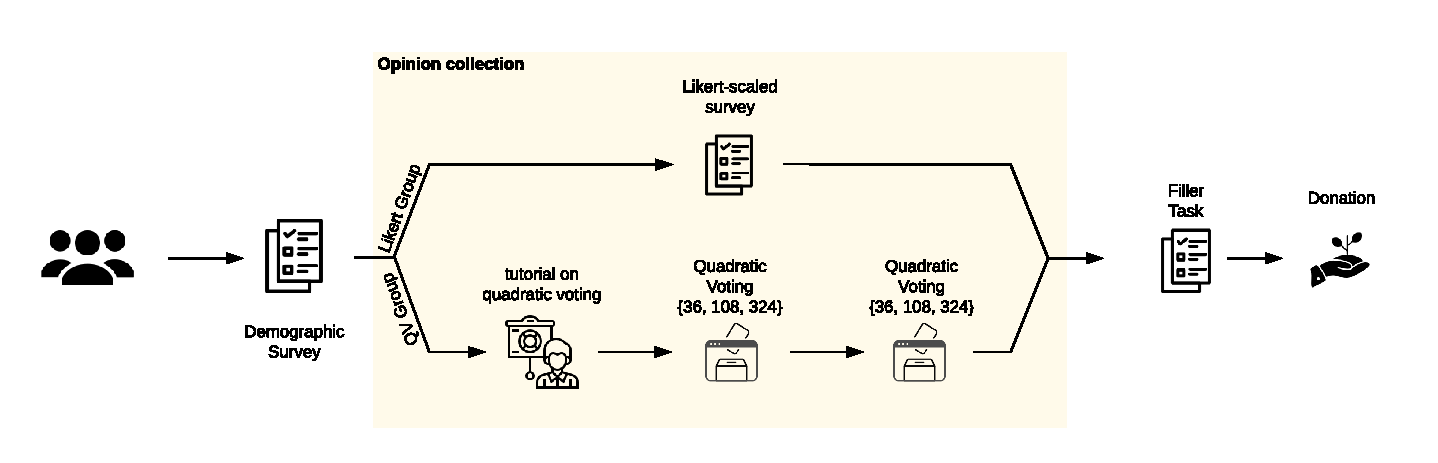
\includegraphics[width=\textwidth, keepaspectratio=true]{content/image/exp1_flow.pdf}
%     \caption{
%         Experiment one conducted between and within subjects. Participants were divided into two groups. Participants that took the upper path are the Likert Group, who expressed attitudes of various social causes through a five-point Likert Survey. The alternative is the QV group who replied attitudes through two QV surveys, each with a different combination among the three possible votes: $36$, $108$, or $324$ credits.
%     }
%     \Description[Image describing the flow for experiment 1]{Image describing the flow for experiment 1}
%     \label{fig:exp1_image_flow}
% \end{figure}

% At a high level, 
% we summarize the experiment flow 
% in Graph \ref{fig:exp1_image_flow}.
% The experiment consisted of four steps:
% To begin the experiment, 
% participants filled out the demographic survey.
% Based on the demographics,
% participants completed one form of opinion collection,
% highlighted as the yellow box
% in Graph \ref{fig:exp1_image_flow}.
% After that, 
% participants filled out another survey,
% the distraction survey,
% to divert their attention before they complete the final task.
% The final task asked participants to donate.
% Now we explain each section in detail.

% Before starting the experiment,
% participants were told that 
% this study aims to understand their opinions 
% toward social causes and will be asked to complete a donation task.
% During the demographic survey, 
% we collected the participant's gender, ethnicity, age range, household income level, 
% education level, and current occupation.
% Based on the age and education level,
% we divided participants into seven groups
% and made sure each group contained the same distribution
% as the US 2019 census.
% These seven groups can be further categorized as
% the Likert Group (Group 1) and the QV Group (Group 2 to 7).
% The Likert Group, shown as the upper path in the shaded area of Graph \ref{fig:exp1_image_flow}, 
% revealed their opinion using a Likert survey.
% The QV Group, shown as the lower path in the shaded area of Graph \ref{fig:exp1_image_flow}, 
% revealed their opinions by completing two QVs, each with different numbers of voice credit.
% We divided the QV Group into six subgroups
% to answer research question three, 
% which is whether the number of voice credits impacts the outcome.
% These two voice credits that participants experience 
% are drawn from three possible values: $N \times O$, $N^{1.5} \times O$, $N^2 \times O$, 
% where $N$ is the number of options in the survey, 
% and $O$ is the number of levels, 
% excluding neutral on the Likert survey. %not sure if this is clear
% In our case, with nine options ($N=9$) and
% used a five-point Likert survey ($O=4$), 
% the three values would be $36$, $108$, and $324$.
% With these three possible values, 
% we choose two for each of the six subgroups.

% In the Likert group, 
% the survey looks identical to a typical five-point Likert survey.
% We assume participants have prior knowledge in Likert surveys.
% Participants were presented with the nine societal causes, 
% and were asked the importance each of these causes: 
% With options ranging from ``Very important'' to ``Very Unimportant.''

% In the QV group, 
% participants were asked to watch 
% a prerecorded tutorial video of QV's concept 
% and how to operate the QV interface.
% Participants are granted unlimited time 
% to interact with a demo QV interface. 
% This process is demonstrated as 
% ``tutorial on quadratic voting'' 
% in Graph \ref{fig:exp1_image_flow}.
% To ensure that participants paid attention to the video and understood QV, 
% they were asked to answer at least three of the five multiple-choice questions 
% correctly to continue with the survey.
% Once participants passed the quiz, 
% participants will be given voice credits of either 36, 108, or 324.
% They will vote in QV using these voice credits 
% with the nine options identical to those in the Likert Group.
% Participants would repeat this action using a different set of voice credits.
% These two QVs are shown as two QV icons in Graph \ref{fig:exp1_image_flow}.

% After both groups of participants completed their surveys in the opinion collection stage, 
% they finish a short answer question
% that allowed them to express their thoughts 
% related to another set of societal issues.
% These societal issues are unrelated in the previous stage,
% and are designed to distract participants.
% We do not want participants to connect their survey responses
% to interfere with their behaviors during the donation task.

% Finally, 
% we ask participants to perform a donation in the final stage.
% This task presented nine organizations,
% each referring to one of the nine societal causes
% that we listed during the opinion collection phase.
% Participants can donate 
% any amount to any of the listed organizations
% without exceeding a total of 35 dollars.
% To ensure incentive compatibility, 
% participants do not donate imaginatively.
% Participants are aware that every one in 70 participants would win 35 US dollars.
% Assuming winning the 35 US dollars, 
% the participants were asked 
% if they would want to donate some money 
% to any of the nine charity groups.
% Participants are also aware that 
% they keep the remaining amount of undonated money 
% if they win the lottery.
% Further, participants are aware that 
% the research team will match one dollar to each one dollar 
% they donated to an organization.
% \tc{We need to justify why we matched}
% This setup means the donation carried an underlying cost.

% To minimize the difference across groups in the study, 
% we use the same prompt across Likert survey, QV, and the donation task.
% We explicitly tell the participants that 
% there are limited resources in the society, 
% and people have different preferences 
% in how resources should be allocated and ask the participants, 
% ``What societal issues need more support?''

% To ensure that the nine societal causes 
% covered a broad spectrum of categories.
% We used the categorization of charity groups on Amazon Smile, 
% a popular donation website that has accumulated over 100 million dollars of donations, 
% as our topics of the societal causes.
% The categories include:
% \begin{enumerate}[label={},leftmargin=\parindent]
%     \item (1) Pets and Animals
%     \item (2) Arts, Culture, and Humanities
%     \item (3) Education
%     \item (4) Environment
%     \item (5) Health
%     \item (6) Human Services
%     \item (7) International
%     \item (8) Faith and Spiritual
%     \item (9) Veteran
% \end{enumerate}
% Within each of these categories, 
% we select one charity organization from Amazon Smile 
% as the representation of the subject matter used in the donation task.

% \subsection{System Design}
% We use Python Flask for the back-end, Angular for front-end, 
% and MongoDB for database storage to construct the voting system. 
% The experiment source code is publicly available \footnote{Not yet public}, 
% and so is the QV interface as a stand-alone repository \footnote{https://github.com/hank0982/QV-app}.

% \begin{figure}[htpb]
%     \centering
%     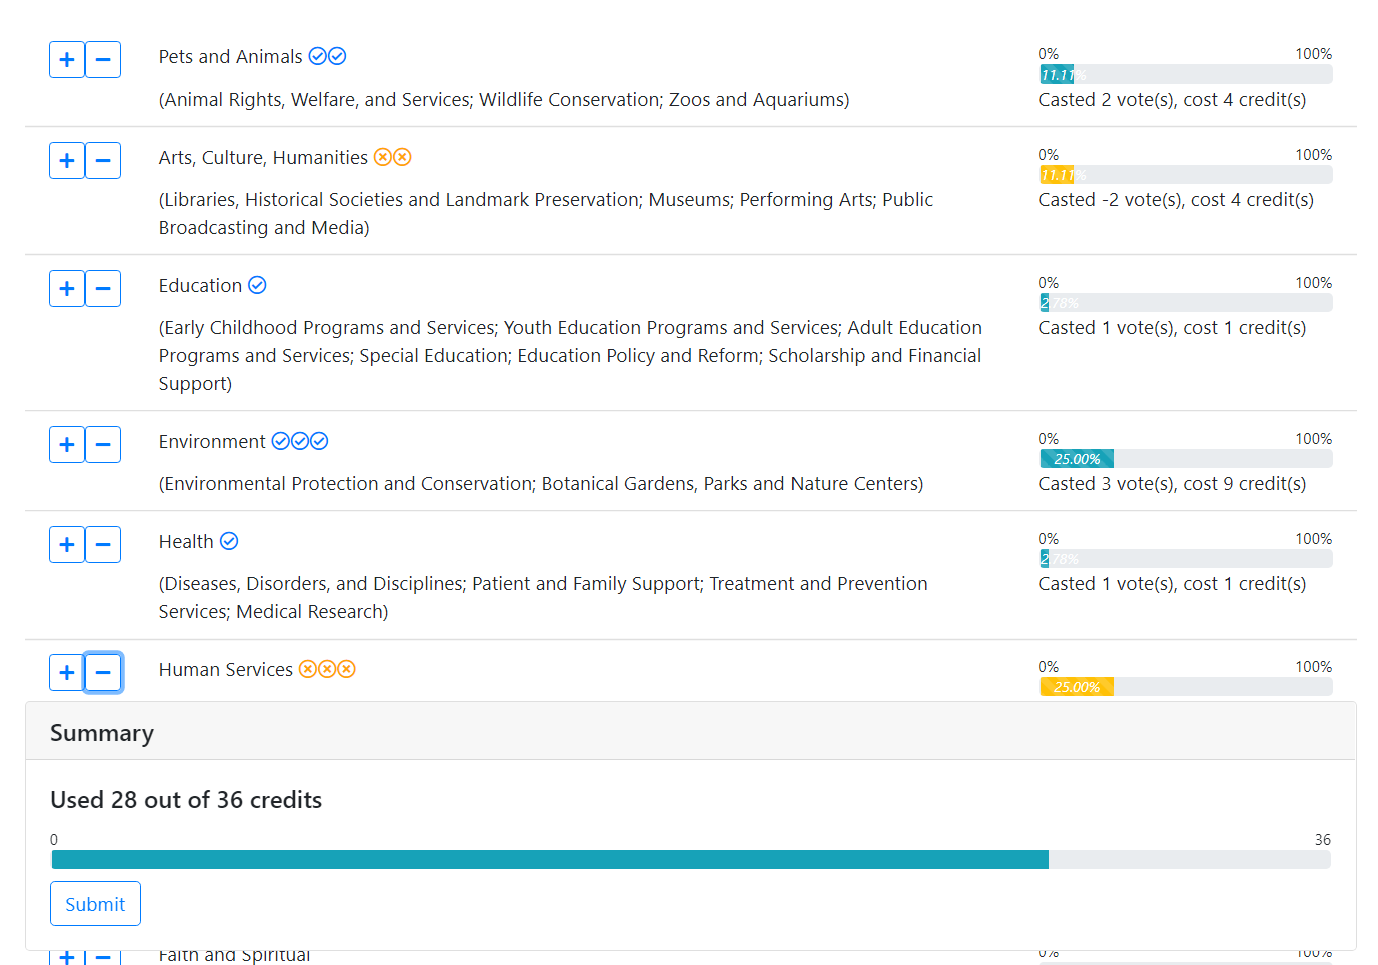
\includegraphics[width=0.7\textwidth, keepaspectratio=true]{content/image/qv-donation.png}
%     \caption{
%         The QV voting interface used across both experiments. 
%         We omit the prompt in this figure.
%         After mutiple iterations (details in the Appendeix), 
%         the interface allows participants to vote, 
%         with real time feedback of how the votes allocats. 
%         The progress bar implementation 
%         were inspired by knapsack voting interface by \textcite{goel2015knapsack}.
%     }
%     \label{fig:qv_donation}
% \end{figure}

% The QV interface, is shown in Figure \ref{fig:qv_donation}.
% The body section is the voting panel
% that contained all options to vote for.
% To the left of each option, 
% participants vote using the plus and minus buttons.
% Buttons are disabled 
% if the number of voice credits 
% does not permit the next vote.
% A bar on the right of the option 
% shows the proportion of voice credits 
% used to that option with text associated with the visual.
% The different colors and the icons 
% to the right of each option 
% exhibits the number of for or against 
% that currently devoted to an option.
% The summary panel always 
% floats at the bottom of the page 
% to ensure visibility.
% A progress bar shows the number of voice credits 
% that the participants have and had not used.\par